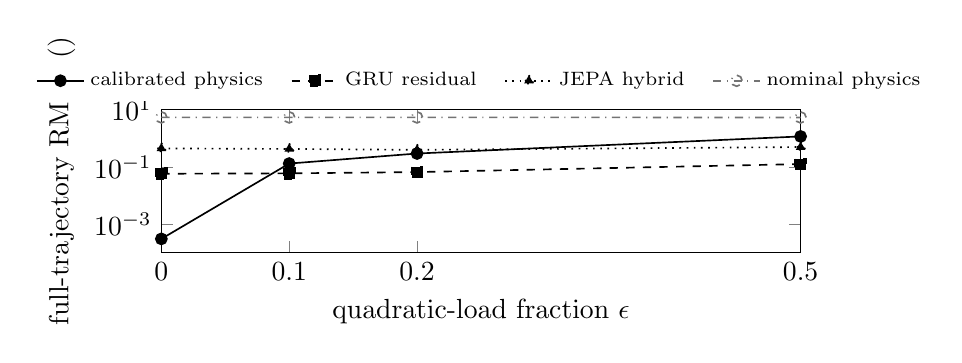
\begin{tikzpicture}
\begin{axis}[width=0.80\textwidth,height=0.28\textwidth,xlabel={quadratic-load fraction $\epsilon$},ylabel={full-trajectory RMSE (\si{\radian\per\second})},xmin=0,xmax=.5,ymin=1e-4,ymax=10,ymode=log,grid=none,minor y tick num=1,legend style={font=\scriptsize,draw=none,at={(0.5,1.06)},anchor=south,legend columns=4,/tikz/every even column/.append style={column sep=0.8em}},xtick={0,.1,.2,.5}]
\addplot[black,solid,semithick,mark=*] coordinates {(0,.0003) (.1,.1302) (.2,.2925) (.5,1.1603)};\addlegendentry{calibrated physics}
\addplot[black,dashed,semithick,mark=square*] coordinates {(0,.0573) (.1,.0591) (.2,.0655) (.5,.1248)};\addlegendentry{GRU residual}
\addplot[black,dotted,semithick,mark=triangle*] coordinates {(0,.4412) (.1,.4227) (.2,.3933) (.5,.4933)};\addlegendentry{JEPA hybrid}
\addplot[black!55,dashdotted,semithick,mark=o] coordinates {(0,5.3921) (.1,5.3884) (.2,5.3839) (.5,5.3620)};\addlegendentry{nominal physics}
\end{axis}
\end{tikzpicture}
